% Fig. 3 -- admission per engine and the verdicts of the static Contract B rule (column width, Section 5)
\begin{figure}[htbp]
  \centering
  \subcaptionbox{The funnel of Table~\ref{tab:funnel} per engine\label{fig:funnelengine}}{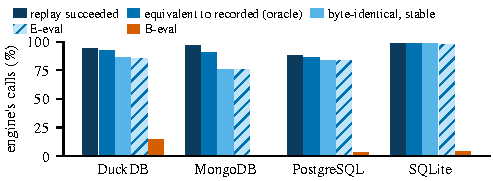
\includegraphics[width=\columnwidth]{figures/fig3a_funnel_engine}}
  \subcaptionbox{Verdicts of the static Contract B rule\label{fig:verdicts}}{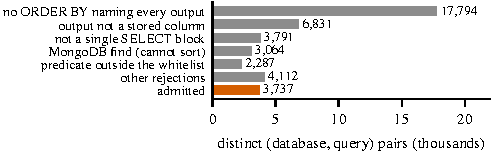
\includegraphics[width=\columnwidth]{figures/fig3b_b_verdicts}}
  \caption{Admission by engine and by rule. (a) Share of each engine's calls that passes each cumulative gate of Table~\ref{tab:funnel}. It covers the 76,141 calls with a replay outcome, and Table~\ref{tab:workload} gives the totals.
  MongoDB's B-eval subset, two calls, is too small to see. (b) Verdict of the static Contract B rule on each of the 41,616 distinct (database, query) pairs. Bars show rejection reasons and the admitted pairs.}
  \label{fig:certify}
  \Description{Two panels. Top: grouped bars per engine showing that most calls of every engine pass the replay, equivalence, byte-identity and E-eval gates, while the B-eval subset is a small share. Bottom: horizontal bars of the number of distinct (database, query) pairs per verdict of the static Contract B rule. The longest bar is the rejection for lacking an ORDER BY that names every output.}
\end{figure}
